\documentclass{standalone}
\usepackage{xcolor}
\usepackage{verbatim}
\usepackage[T1]{fontenc}
\usepackage{graphics}
\usepackage{hyperref}
\newcommand{\code}[1]{\texttt{#1}}
\newcommand{\R}{R}
\newcommand{\pkg}[1]{#1}
\newcommand{\CRANpkg}[1]{\pkg{#1}}%
\newcommand{\BIOpkg}[1]{\pkg{#1}}
\usepackage{amsmath,amssymb,array}
\usepackage{booktabs}
\usepackage{lscape}
\usepackage{bm}
\usepackage{mathrsfs}
\usepackage{graphicx}
\usepackage{tablefootnote}
\usepackage{footmisc}
\usepackage{pdflscape}
\usepackage{enumerate}
\usepackage[shortlabels]{enumitem}
\usepackage{afterpage}
\usepackage{makecell}
\usepackage{capt-of}% or use the larger `caption` package
\usepackage{subfig}
\usepackage{listings}
\usepackage{adjustbox}
\usepackage{multirow}
\usepackage{booktabs}
\usepackage{tikz}
\usetikzlibrary{matrix,calc,shapes,arrows}
\usetikzlibrary{shapes.multipart} 
\tikzset{
  treenode/.style = {shape=rectangle, rounded corners,
                     draw,align=center,
                     top color=white,
                     text width = 4cm,
                     inner sep=2ex,
                     anchor=center},
  input/.style = {align=center, text width=4.5cm},
  decision/.style = {treenode, diamond, inner sep=3pt},
  action/.style = {treenode, circle, inner sep=1pt,
                     text width = 2.5cm},
  root/.style     = {treenode},
  env/.style      = {treenode},
  ginish/.style   = {root},
  dummy/.style    = {circle,draw},
  ar/.style={->,>=latex}
}
\tikzset{connect/.style={rounded corners=#1,
        to path= ($(\tikztostart)!-#1!(\tikztotarget)!-#1!-90:(\tikztotarget)$) -- ($(\tikztotarget)!-#1!(\tikztostart)!-#1!90:(\tikztostart)$) --
        ($(\tikztotarget)!-#1!(\tikztostart)!#1!90:(\tikztostart)$) -- ($(\tikztostart)!-#1!(\tikztotarget)!-#1!90:(\tikztotarget)$) -- cycle (\tikztotarget)
}}
\tikzset{connect/.default=4mm}
\begin{document}
\nopagecolor
\centering

\resizebox{\textwidth}{!}{%
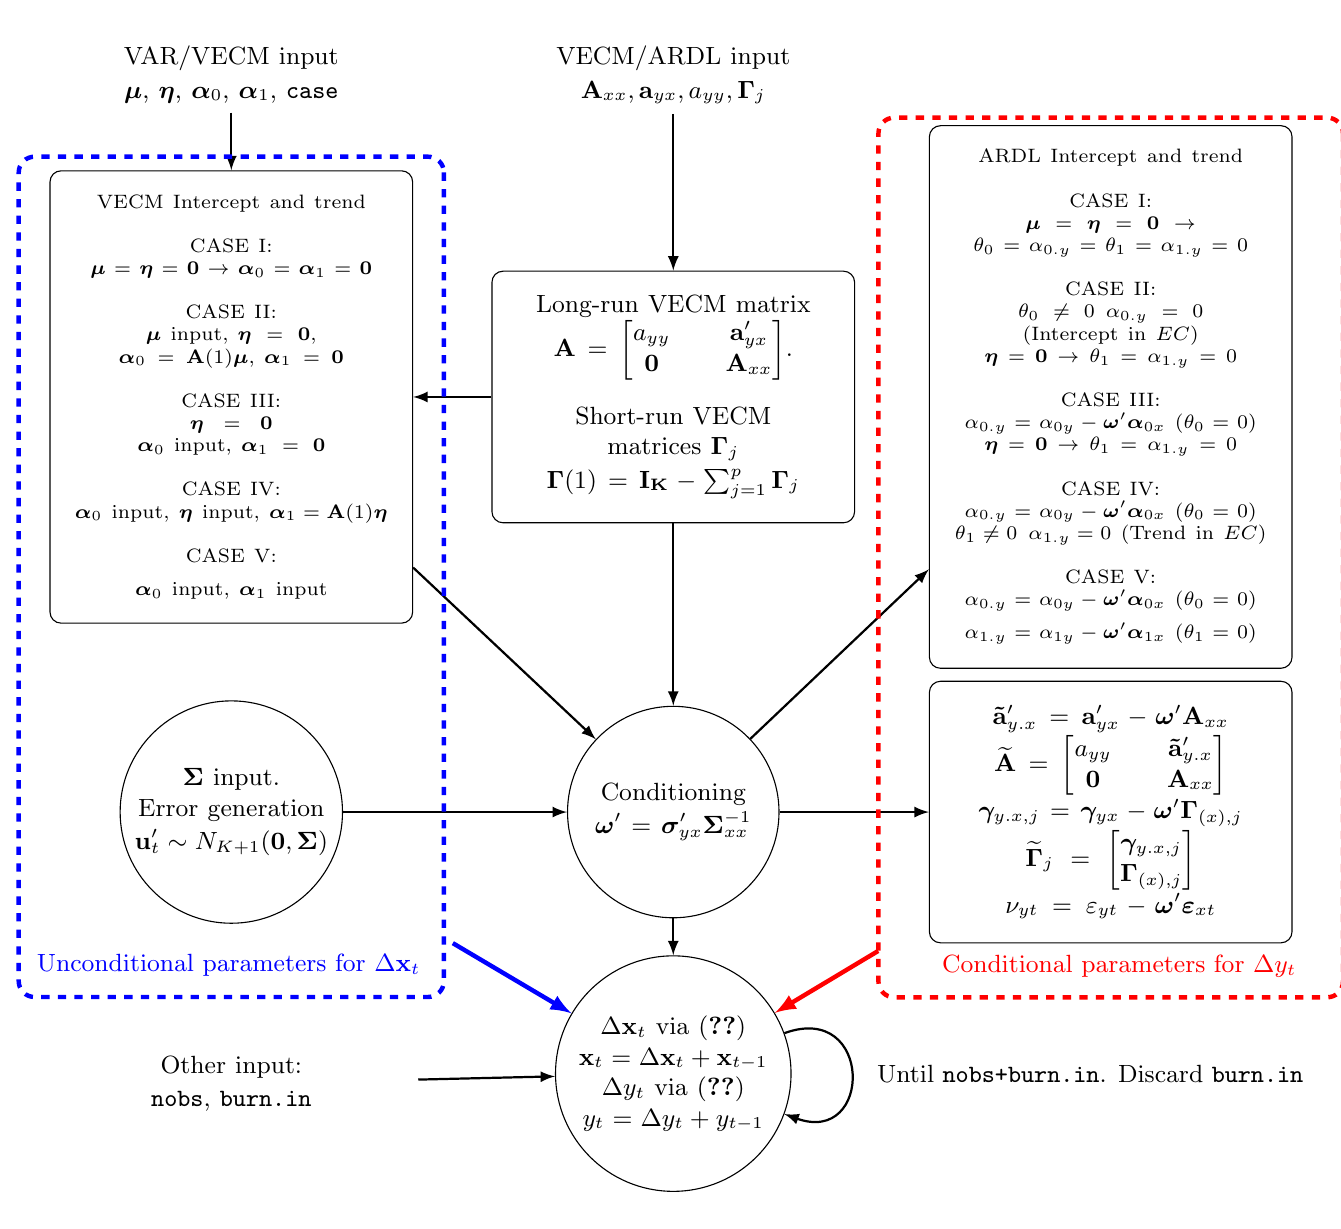
\begin{tikzpicture}[-latex][scale=0.3]
  \matrix (chart)
    [
      matrix of nodes,
      column sep      = 2.5em,
      row sep         = 1ex,
      row 2/.style = {nodes={decision}},
      row 5/.style = {nodes={env}}
    ]
    {  %first row
       |[input]| {\small VAR/VECM input\\ $\boldsymbol \mu$, $\boldsymbol \eta$, $\boldsymbol\alpha_0$, $\boldsymbol\alpha_1$, \texttt{case}}
       &
       |[input]| {\small VECM/ARDL input\\ $\mathbf A_{xx},\mathbf a_{yx},a_{yy},\boldsymbol{\Gamma}_j$}&
       \\
       %second row
       |[treenode]|{\scriptsize  VECM
       Intercept and trend\\
       \phantom{x}\\
       CASE I:\\  $\boldsymbol{\mu}=\boldsymbol{\eta}=\mathbf 0\rightarrow
        \boldsymbol\alpha_0 = \boldsymbol\alpha_1 = \mathbf 0$     \\
       \phantom{x}\\
       CASE II:\\ 
       $\boldsymbol{\mu}$ input, $\boldsymbol\eta=\mathbf 0$, $\boldsymbol\alpha_{0} =  \mathbf A(1) \boldsymbol{\mu}$, $\boldsymbol\alpha_1 = \mathbf 0$\\
        \phantom{x}\\
        CASE III:\\
       $\boldsymbol\eta=\mathbf 0 $ \\
       $\boldsymbol{\alpha}_{0}$ input, $\boldsymbol{\alpha}_1 = \mathbf 0$\\ 
       \phantom{x}\\
       CASE IV:\\
       $\boldsymbol{\alpha}_{0}$ input, $\boldsymbol{\eta}$ input, $\boldsymbol{\alpha}_1 =\mathbf A(1)\boldsymbol{\eta}$\\
       \phantom{x}\\
       CASE V:\\
       $\boldsymbol{\alpha}_{0}$ input, $\boldsymbol{\alpha}_1$ input
       \normalsize}&
       |[treenode]| {\small Long-run VECM matrix 
       $\mathbf A = 
       \begin{bmatrix} {a_{yy}} & {\mathbf{a}_{yx}'} \\
       {\mathbf 0} & {\mathbf{A}_{xx}}  
       \end{bmatrix}$.\\
       \phantom{x}\\
       Short-run VECM matrices 
       $\boldsymbol\Gamma_j$ \\
       $\boldsymbol\Gamma(1) = \mathbf{I_K}-\sum_{j=1}^p\boldsymbol\Gamma_j$}&
       |[treenode]|{\scriptsize  ARDL
       Intercept and trend\\
       \phantom{x}\\
       CASE I:\\  $\boldsymbol{\mu}=\boldsymbol{\eta}=\mathbf 0\rightarrow$\\
        $\theta_0=\alpha_{0.y} = \theta_1=\alpha_{1.y} = 0$\\
       \phantom{x}\\
       CASE II:\\
       $\theta_0\neq 0 \enspace \alpha_{0.y} = 0$ (Intercept in $EC$)\\
       $\boldsymbol\eta=\mathbf 0 \rightarrow \theta_1 =\alpha_{1.y}= 0$\\
        \phantom{x}\\
        CASE III:\\
        $\alpha_{0.y}=\alpha_{0y}-\boldsymbol\omega'\boldsymbol\alpha_{0x}$ $(\theta_0 =  0)$\\
       $\boldsymbol\eta=\mathbf 0 \rightarrow \theta_1 =\alpha_{1.y}= 0$\\ 
       \phantom{x}\\
       CASE IV:\\
       $\alpha_{0.y}=\alpha_{0y}-\boldsymbol\omega'\boldsymbol\alpha_{0x}$ $(\theta_0 =  0)$\\
       $\theta_1\neq 0 \enspace \alpha_{1.y} = 0$ (Trend in $EC$)\\
       \phantom{x}\\
       CASE V:\\
       $\alpha_{0.y}=\alpha_{0y}-\boldsymbol\omega'\boldsymbol\alpha_{0x}$ $(\theta_0 =  0)$\\
       $\alpha_{1.y}=\alpha_{1y}-\boldsymbol\omega'\boldsymbol\alpha_{1x}$ $(\theta_1 =  0)$
       \normalsize}
       \\
       %third row
       |[action]| {\small $\boldsymbol{\Sigma}$ input.\\ Error generation\\
       $\mathbf u_t'\sim N_{K+1}(\mathbf 0,\boldsymbol\Sigma)$
       \normalsize}&
       |[action]| {\small Conditioning\\
       $\boldsymbol\omega'=
       \boldsymbol\sigma_{yx}'\boldsymbol\Sigma_{xx}^{-1}$
       \normalsize}&
       |[treenode]|{\small $\mathbf {\tilde{a}}_{y.x}'=\mathbf a_{yx}'-\boldsymbol\omega'\mathbf A_{xx}$\\
       $\widetilde{\mathbf A} =
       \begin{bmatrix}
       {a_{yy}} & \mathbf{\tilde{a}}'_{y.x}\\
       {\mathbf 0} & {\mathbf{A}_{xx}}  
       \end{bmatrix}$\\
       $\boldsymbol\gamma_{y.x,j}=
       \boldsymbol\gamma_{yx}-\boldsymbol\omega'\boldsymbol\Gamma_{(x),j}$\\
       $\widetilde{\boldsymbol\Gamma}_j =
       \begin{bmatrix}
       \boldsymbol{\gamma}_{y.x,j}\\
       \boldsymbol\Gamma_{(x),j}
       \end{bmatrix}$\\
       $\nu_{yt}=\varepsilon_{yt}-\boldsymbol\omega'\boldsymbol\varepsilon_{xt}$
       \normalsize}\\
        |[input]| {\small Other input:\\
        \texttt{nobs}, \texttt{burn.in}}
       &
       |[action]| {\small $\Delta \mathbf x_t$ via \eqref{eq:marg}\\
       $\mathbf x_t = \Delta \mathbf x_t + \mathbf x_{t-1} $\\
       $\Delta y_t$ via \eqref{eq:ardl}\\
       $y_t = \Delta y_t + y_{t-1} $\\
       \normalsize}&\\
       };
       \draw[thick]
		 (chart-1-1) ->  (chart-2-1);
       \draw[thick]
		 (chart-1-2) -> (chart-2-2);
       \draw[thick]
		 (chart-2-2) -> (chart-2-1);
       \draw[thick]
		 (chart-2-1) -> (chart-3-2);
       \draw[thick]
		 (chart-2-2) -> (chart-3-2);
       \draw[thick]
		 (chart-3-1) -> (chart-3-2);
       \draw[thick]
		 (chart-3-2) -> (chart-2-3);
       \draw[thick]
		 (chart-3-2) -> (chart-3-3);
    \begin{scope}[transform canvas={yshift=1.7em}]
       \draw[red,dashed,ultra thick] (chart-2-3) to[connect=29.5mm,rounded corners=2mm] (chart-3-3);
    \end{scope}
    \begin{scope}[transform canvas={yshift=1em}]
       \draw[blue,dashed,ultra thick] (chart-2-1) to[connect=27mm,rounded corners=2mm] (chart-3-1);
    \end{scope}
       \draw[blue,ultra thick,shorten < = 1.85cm] (chart-3-1) edge node[left=0.75cm,pos=0.67]{\small Unconditional parameters for $\Delta\mathbf x_t$\normalsize} (chart-4-2);
       \draw[red,ultra thick,shorten < = 0.75cm] (chart-3-3) edge node[right=1cm,pos=0.5]{\small Conditional parameters for $\Delta y_t$\normalsize} (chart-4-2);
       \draw[thick]
		 (chart-3-2) -> (chart-4-2);
       \draw[thick] (chart-4-2) edge [in=-20, out=20,looseness=3,right=0.2cm] node[right=0.2cm]{\small Until \texttt{nobs+burn.in}. 
       Discard \texttt{burn.in}\normalsize} (chart-4-2);
       \draw[thick]
		 (chart-4-1) -> (chart-4-2);
  \end{tikzpicture}
}
\end{document}
